\subsubsection{Package Game}
The Control's "Game" subsystem is mainly comprised of the event handler for user actions, such as key presses. The classes in this subsystem turn user interactions into Commands given to the Model, or manipulations of the View. This subsystem is the core of the Control part of the MVC architecture, serving as the method by which a user  interacts with the Codenames game.

\paragraph{Detailed Design Diagram}\mbox{}
\begin{figure}[H]
\centering
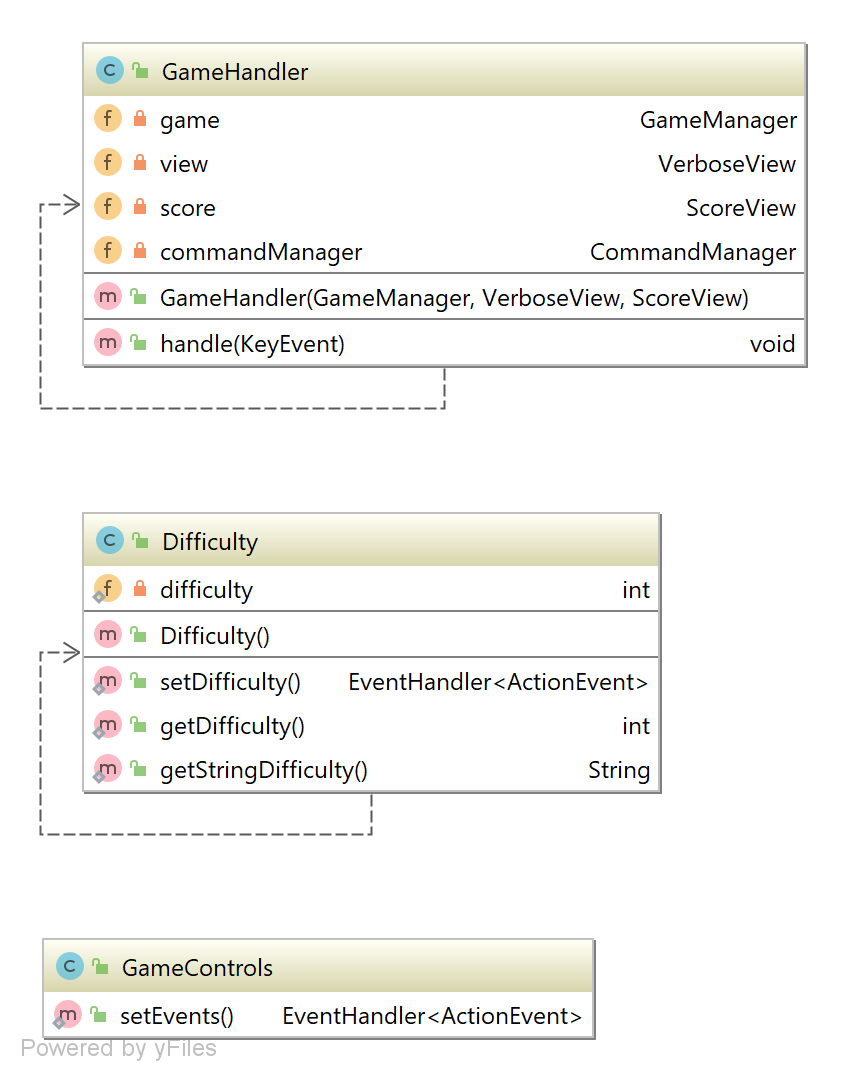
\includegraphics[width=10cm]{Source/Module/Control/Game/Control_Game.png}\caption{UML Diagram of Package Game in Module Control}
\label{Control.Game}
\end{figure}

\paragraph{Class GameHandler}\mbox{}
\begin{tabularx}{\textwidth}{|c||l|X|X|X|}
    \hline
    \cellcolor{lightgray}Class Name & \multicolumn{4}{X|}{GameHandler}\\
    \hline
    \cellcolor{lightgray}Inherits From & \multicolumn{4}{X|}{EventHandler\textlangle{}KeyEvent\textrangle{}}\\
    \hline
    \cellcolor{lightgray}Description & \multicolumn{4}{p{12cm}|}{Main entry point of the program. Engine for running the Codenames game.}\\
    \hline\hline
    
    \cellcolor{lightgray}Attributes & \cellcolor{lightgray}Visibility & \cellcolor{lightgray}Data type & \cellcolor{lightgray}Name & \cellcolor{lightgray}Description\\\cline{2-5}
    \cellcolor{lightgray} & Private & GameManager & game & GameManager object responsible for initializing the game in the constructor.\\\cline{2-5}
    \cellcolor{lightgray} & Private & VerboseView & view & VerboseView object  responsible for initializing the view in the constructor.\\\cline{2-5}
    \cellcolor{lightgray} & Private & ScoreView & score & ScoreView object  responsible for initializing the score in the constructor.\\\cline{2-5}
    \cellcolor{lightgray} & Private & CommandManager & commandManager & CommandManager object  responsible for initializing the commandManager in the constructor as a new object.\\
    \hline\hline
    
    \cellcolor{lightgray}Methods & \cellcolor{lightgray}Visibility & \multicolumn{2}{l|}{\cellcolor{lightgray}Method Name} & \cellcolor{lightgray}Description\\\cline{2-5}
    \cellcolor{lightgray} & Public & \multicolumn{2}{X|}{GameHandler(GameManager game, VerboseView view, ScoreView score)} & Initializes the game, view, and score. Binds the commandManager to a new commandManager object. Shows the score scene.\\\cline{2-5}
    \cellcolor{lightgray} & Public & \multicolumn{2}{X|}{handle(KeyEvent keyEvent)} & When the user presses ENTER, the KeyHandler triggers the playerControl to play the next turn.\\
    \hline
\end{tabularx}

\paragraph{Class Difficulty}\mbox{}
\begin{tabularx}{\textwidth}{|c||l|l|l|X|}
    \hline
    \cellcolor{lightgray}Class Name & \multicolumn{4}{X|}{Difficulty}\\
    \hline
    \cellcolor{lightgray}Inherits From & \multicolumn{4}{X|}{None}\\
    \hline
    \cellcolor{lightgray}Description & \multicolumn{4}{p{12cm}|}{This class is responsible for setting the difficulty of the game.}\\
    \hline\hline
    
    \cellcolor{lightgray}Attributes & \cellcolor{lightgray}Visibility & \cellcolor{lightgray}Data type & \cellcolor{lightgray}Name & \cellcolor{lightgray}Description\\\cline{2-5}
    \cellcolor{lightgray} & Private & int & difficulty & Current difficulty. Default = 0.\\
    \hline\hline
    
    \cellcolor{lightgray}Methods & \cellcolor{lightgray}Visibility & \multicolumn{2}{l|}{\cellcolor{lightgray}Method Name} & \cellcolor{lightgray}Description\\\cline{2-5}
    \cellcolor{lightgray} & Public & \multicolumn{2}{l|}{Difficulty()} & Default constructor.\\\cline{2-5}
    \cellcolor{lightgray} & Public & \multicolumn{2}{l|}{setDifficulty()} & Event Handler that is responsible for setting the game difficulty based on input provided.\\\cline{2-5}
    \cellcolor{lightgray} & Public & \multicolumn{2}{l|}{getDifficulty()} & Retrieves the difficulty level of the game.\\\cline{2-5}
    \cellcolor{lightgray} & Public & \multicolumn{2}{l|}{getStringDifficulty()} & Returns a string representation of the level of difficulty of the game.\\
    \hline
\end{tabularx}
\paragraph{Class GameControls}\mbox{}
\begin{tabularx}{\textwidth}{|c||l|l|l|X|}
    \hline
    \cellcolor{lightgray}Class Name & \multicolumn{4}{X|}{GameControls}\\
    \hline
    \cellcolor{lightgray}Inherits From & \multicolumn{4}{X|}{None}\\
    \hline
    \cellcolor{lightgray}Description & \multicolumn{4}{p{12cm}|}{This class is responsible for handling the events regarding the Restart option or Quit. If Restart has been selected then the program will automatically restart the game and set up a new board.}\\
    \hline\hline
    
    \cellcolor{lightgray}Methods & \cellcolor{lightgray}Visibility & \multicolumn{2}{l|}{\cellcolor{lightgray}Method Name} & \cellcolor{lightgray}Description\\\cline{2-5}
    \cellcolor{lightgray} & Public & \multicolumn{2}{l|}{setEvents()} & Handles events. (Quit, Restart, About)\\\cline{2-5}
    \cellcolor{lightgray} & Public & \multicolumn{2}{l|}{setAbout()} & Handles the about command.\\\cline{2-5}
    \hline
\end{tabularx}
